\section{Sums, Temperature and the Puzzles Revisited}\label{sec:sums}

Most endgames are sums: the position splits into components, and the player to move picks one of them. In this
section we recall two principles for that choice, use them on three puzzles, and ask when adding up the
components gives the same winner as the game on the whole board.

\subsection{Two Principles}

\emph{Principle 1 (number avoidance).} In a sum of numbers and games that are not numbers, if a player can win,
they can win without moving in a number~\cite{WinningWays,Siegel2013}. For the chess player: do not spend a
tempo move in a component whose value is a number while some other component is not a number.

\emph{Principle 2 (the hottest move).} Move in the component with the highest temperature. A switch
$\game{x}{y}$ between numbers $x>y$ has mean $(x+y)/2$ and temperature $(x-y)/2$, the amount each side gains by
moving there first. An infinitesimal such as $\star$, ${\uparrow}$ or $\tinyg{1}$ lies strictly between all
negative and all positive numbers and has temperature $0$. This principle is not universally true, but it holds
in all our examples.

\subsection{The Puzzles Revisited}

Fig.~\ref{fig:puzzles} shows three puzzles on the cylinder, and Table~\ref{tab:puzzles} compares the values
first claimed for them~\cite{Bhattacharjee2025} with the exact ones. As before, we break each position into
smaller games.

\begin{figure*}[!t]
\centering
\begin{subfigure}{0.32\textwidth}
\centering
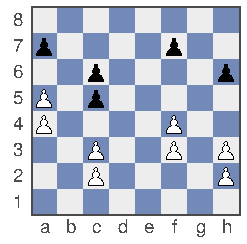
\includegraphics[width=\linewidth]{figures/puzzle71.pdf}
\caption{Puzzle 1: white wins whoever moves first.}
\label{fig:puzzle71}
\end{subfigure}\hfill
\begin{subfigure}{0.32\textwidth}
\centering
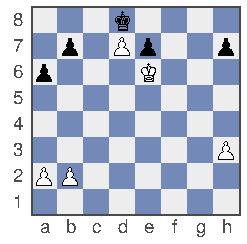
\includegraphics[width=\linewidth]{figures/puzzle72.pdf}
\caption{Puzzle 2: the pawn part is an infinitesimal.}
\label{fig:puzzle72}
\end{subfigure}\hfill
\begin{subfigure}{0.32\textwidth}
\centering
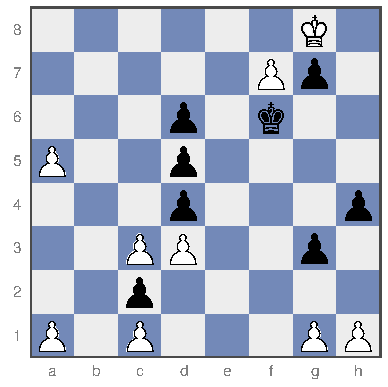
\includegraphics[width=\linewidth]{figures/puzzle73.pdf}
\caption{Puzzle 3 as first drawn: $+\BIG$ (not legal).}
\label{fig:puzzle73}
\end{subfigure}
\caption{Three puzzles (cylinder: files a and h adjacent), Positions 7.1--7.3 of~\cite{Bhattacharjee2025}. Their
exact values are in Table~\ref{tab:puzzles}.}
\label{fig:puzzles}
\end{figure*}

\begin{table}[!t]
\centering
\caption{The Puzzles of Fig.~\ref{fig:puzzles}: Claimed and Exact Values \lab{C2}}
\label{tab:puzzles}
\begin{tabular}{@{}lll@{}}
\toprule
Part & Claimed~\cite{Bhattacharjee2025} & Exact \\
\midrule
1: c-file & $\pm1$ & $\pm1$ \\
1: f-file & $\game{\game{2}{1}}{0}$ & the same (mean $3/4$) \\
1: files h, a & $1$ & $\game{+\BIG}{\star}$ (hot) \\
1: total & $1\pm1+\game{\game{2}{1}}{0}$ & white wins either way \\
2: pawns & $\pm1$ & infinitesimal, mean $0$ \\
2: kings & $0$ & not a zugzwang \\
3: files c, d & $1$ & $\tinyg{1}$ \\
3: total & $2$ & $+\BIG$ before any move \\
\bottomrule
\end{tabular}
\end{table}

\emph{Puzzle 1} (Fig.~\ref{fig:puzzle71}) has three components. On the c-file the first player wins: white
(Left) c3--c4 leaves $1$ and black (Right) c5--c4 leaves $-1$, so $G=\game{1}{-1}=\pm1$. On the f-file white's
f4--f5 leaves $\game{2}{1}$ (white can go on with f5--f6 and keep two spare moves with the f3 pawn, while
black's f7--f6 leaves white one), and black's best, f7--f5, locks the file at $0$. Thus
$G=\game{\game{2}{1}}{0}$, with mean $3/4$, as first found. The earlier analysis goes wrong on files h and a.
White's a5--a6 still wins outright, but black, moving first, plays h6$\times$a5 across the seam and leaves
$\star$, not a loss. So $G=\game{+\BIG}{\star}$: this part is hot, not the number $1$.

The total is still a white win whoever moves first, but for a different reason. By Principle~2 the h/a
component is by far the hottest. White to move plays a5--a6 and wins. Black to move must take on a5 at once,
since any other move allows a5--a6. Then white plays c3--c4 in the next hottest component, and
$1+\star+\game{\game{2}{1}}{0}$ is a white win whoever moves next.

\emph{Puzzle 2} (Fig.~\ref{fig:puzzle72}) has one pawn component, on files h, a and b. The earlier walk-through
finds the right first moves, h3--h4 for white and a6--a5 for black, and the right outcome: whoever moves first
wins. But the value is not $\pm1$; it is an infinitesimal with mean $0$ and temperature $0$. In a sum this
matters: a $\pm1$ would demand an early move, while by Principle~2 this component waits until every hot one is
settled. The king group is that of Fig.~\ref{fig:kinggroup72}, frozen for black only, so with black to move
the model's verdict rests on a final white king move that in chess need not lose. The full ten-man position is
beyond the tablebases, and its real result is open.

\emph{Puzzle 3} (Fig.~\ref{fig:puzzle73}) cannot arise in chess, since four white pawns stand on the first rank.
As drawn it is decided before anyone moves, because the pawns on a5 and f7 are already passed; its king group
is not a tr\'ebuchet either, because f7--f8 promotes. The component on files c and d is still instructive (the
pawns on c1 and c2 block each other). White's best move, c3$\times$d4, leaves $0$. Black's only move is
d4$\times$c3, after which white must answer d3--d4 to lock the files at $0$: if black moved there again,
d5--d4 would leave black the spare move d6--d5, which is $-1$. Thus
\[
G=\ggame{0}{0\mid -1}=\tinyg{1},
\]
a positive infinitesimal, not $1$. A legal copy one rank up, \pos{W c2 c4 d4 / B c3 d5 d6 d7}, has the same
value. In all three puzzles the earlier walk-throughs pick the right winner; what changes is the value, and with
it how each component behaves in a larger sum.

\subsection{When Is the Sum Model Right?}\label{sec:sums-hss}

In chess the first passed pawn ends the game. In a sum it does not: a component with a passed pawn becomes the
integer $\pm\BIG$ and play goes on elsewhere, so a $+\BIG$ can cancel a $-\BIG$. The smallest example is
$\game{\BIG}{0}+\game{0}{-\BIG}$. In chess whoever moves first makes a passed pawn and wins, but the sum is $0$,
a second-player win, for every value of $\BIG$ \lab{P}. We write $S(X)$ for the sum model of a pawn position $X$
and $W(X)$ for the whole-board game, which ends at the first passed pawn anywhere.

\begin{definition}[Hereditary sum safety]\label{def:hss}
A component carries a \emph{threat} for a side if some position reachable from it gives that side a passed
pawn. A position $X$ is \emph{hereditarily sum-safe} (HSS) if no position reachable from $X$ before the first
passed pawn, $X$ included, has two different components that carry threats for opposite sides.
\end{definition}

\begin{theorem}[Sum safety; \lab{P}]\label{thm:hss}
Suppose that $X$ is HSS, that no position with two or more components has a usable en passant right
(condition (E)), and that $\BIG$ exceeds the number of moves either side can make. Then $S(X)$ and $W(X)$ have
the same outcome.
\end{theorem}

\begin{proof}[Proof sketch]
The models can differ only after a passed pawn appears, say for white. By HSS no other component can then give
black a passed pawn, so in the sum white wins by moving in its $+\BIG$ every turn while black runs out of its
fewer than $\BIG$ moves. Induction over the game tree, with (E) to match the moves, gives the theorem.
\end{proof}

In a random sample of $1{,}500$ positions, all $1{,}297$ HSS ones agree. With $\BIG=256$ the move bound always
holds on the 8-rank board, since a side has at most eight pawns and each moves at most six times. The theorem is
about outcomes, not values: a spare move in one component survives a passed pawn in another only in the sum.
Condition (V4) of Theorem~\ref{thm:validity} is the same condition beside a king group. Neither HSS nor (E) can
be dropped.

\begin{figure}[!t]
\centering
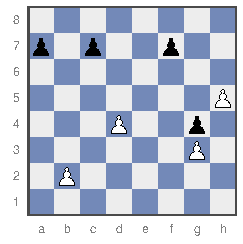
\includegraphics[width=0.5\columnwidth]{figures/sum_counter.pdf}
\caption{Position \pos{W b2 d4 g3 h5 / B a7 c7 f7 g4} (cylinder: files a and h adjacent; en passant off). It is
one component, yet the sum model says that black wins while the whole-board game is a first-player win.}
\label{fig:sum_counter}
\end{figure}

\begin{proposition}[\lab{C2}]\label{prop:sumcounter}
A test of the top-level components alone is not sufficient. On the 8-file cylinder with en passant off,
$X=$\,\pos{W b2 d4 g3 h5 / B a7 c7 f7 g4} (Fig.~\ref{fig:sum_counter}) is a single component, spanning files f
to d across the seam, so such a test passes it. Yet $S(X)$ is a black win whoever starts, while $W(X)$ is a
first-player win.
\end{proposition}

The trouble comes from sums that appear only later in the tree, where components with threats for opposite
sides meet, so the position is not HSS.

\begin{proposition}[\lab{C1}]\label{prop:condE}
Without (E) the sum can be wrong, even in outcome. On the flat $6\times6$ board take \pos{W a4 f4 / B b4 e5},
where white has just played a2--a4, so that black may take b4$\times$a3 en passant on this move only. The whole
board is $\game{0}{-4,\,-3\pm2}$, a first-player win, while the sum of its two components is
$\game{-1\star}{-5\star}$, a black win.
\end{proposition}

In the sum, the en passant right survives moves made in the other component, which chess forbids.

\emph{Two models.} Our CGT engine follows Elkies~\cite{Elkies1996} and adds up components. A separately
written whole-board solver never splits the board and ends the game at the first passed pawn; with splitting
switched off, our engine matches it on every disagreeing case tested. The two models agree on every headline
value of this paper: the $1/8$ and $\upsec\star$ positions in all nine settings, and the seven-pawn $\nim{2}$ under the count rule with the e.p.-aware test. Elsewhere they can differ,
even in outcome: under the opponent race rule with the e.p.-aware test, \pos{W a3 b3 c2 e2 / B a6 c5 d5 e3} is
${\Uparrow}$ as a sum of components but $\nim{2}$ on the whole board. Whenever the two models differ, we say which
one we mean.
